\section{Security Assessment}
\label{appendix:securityassesment}
\subsection{Risk Identification}
\subsubsection{Asset Identification}
By browsing through our setup and documentation, we identified the following list of assets:
\begin{itemize}
    \item Web application
    \item Public GitHub repository
    \item Digital Ocean servers
    \item Tools
    \begin{itemize}
        \item Ansible
        \item Code Climate
        \item Docker, Docker Compose \& Docker Swarm
        \item GitHub Actions
        \item Grafana
        \item Linters
        \item Loki
        \item Pulumi
        \item SonarCloud
    \end{itemize}
\end{itemize}
\subsubsection{Threat Source Identification}
To help us identify possible threats to the system, we have consulted the OWASP \textit{Top 10 Web Application Security Risks}\cite*{OWASP}, which describes the following threats:
\begin{enumerate}
    \item Broken Access Control
    \item Cryptographic Failures
    \item Injection Attacks
    \item Insecure Design
    \item Security Misconfiguration
    \item Vulnerable and Outdated Components
    \item Identification and Authentication Failures
    \item Software and Data Integrity Failures
    \item Security Logging and Monitoring Failures
    \item Server Side Request Forgery
\end{enumerate}
\subsubsection{Risk Scenario Construction}
Based on the information gathered from the two previous steps, we have constructed the following risk scenarios and outlined which of the OWASP top 10 risks affect the scenario:
\begin{enumerate}
    \item \textbf{\underline{URL Tampering}}

    The attacker can construct a URL in the \textbf{web application} with a user ID, such that they can bypass login and are able to write a message from another user’s account.

    This would be an issue of \textit{Broken Access Control} and \textit{Server Side Request Forgery}.
    \item \textbf{\underline{Log Injection}}

    The attacker can fabricate log information via an injection attack in the \textbf{web application} as a means to hide their activity and ill-intentioned actions.

    This would be an issue of \textit{Security Logging and Monitoring Failures} and \textit{Injection Attacks}.
    \item \textbf{\underline{Password Brute Forcing}}

    The attacker can brute force login credentials in the \textbf{web application} by taking advantage of no timeouts and a weaker hash implementation.

    This would be an issue of \textit{Cryptographic Failures} and \textit{Identification and Authentication Failures}.
    \item \textbf{\underline{Depricated Dependencies}}

    The attacker can identify weak, outdated or depricated tools and dependencies in the system's CI/CD pipeline via \textbf{GitHub Actions}, which is publicly availble through the \textbf{GitHub repository}.

    This would be an issue of \textit{Vulnerable and Outdated Components} and \textit{Software and Data Integrity Failures}.
    \item \textbf{\underline{Open Ports}}

    The attacker can scan the public IP addresses of the \textbf{Digital Ocean} servers to find unnecessarily or unexpectedly open ports with known vulnerabilities, which can be exploited in further attacks.

    This would be an issue of \textit{Security Misconfiguration}.
    \item \textbf{\underline{SQL Injection}}

    The attacker can target the login page of the \textbf{web application} with SQL-injection attacks to strike the database.

    This would be an issue of \textit{Injection Attacks}.
    \item \textbf{\underline{Exposed Secrets}}

    The attacker can get access to the system, or associated tools, via secrets found written in the code in the public \textbf{GitHub repository}.

    This would be an issue of \textit{Identification and Authentication Failures} and \textit{Security Misconfiguration}.
\end{enumerate}
\subsection{Risk Analysis}
\subsubsection{Likelihood Analysis}
Likelihood will be graded on the following scale:\{Rare, Unlikely, Possible, Likely, Certain\} with \textit{Rare} being the least severe and \textit{Certain} being the most severe.
\begin{enumerate}
    \item \textbf{\underline{URL Tampering}}

    We examined the different URLs on the web application and could not find any where the IDs or login parameters were exposed. Therefore we deemed the likelihood to be \textbf{Unlikely}.
    \item \textbf{\underline{Log Injection}}

    We received warnings from SonarCloud that we had logging vulnerabilities in our code several different places. Therefore we deemed the likelihood to be \textbf{Likely}.

    \item \textbf{\underline{Password Brute Forcing}}

    We currently do not have any measures in place to combat brute force attacks and no password requirements for the users when signing up. Therefore we deemed the likelihood to be \textbf{Possible}.
    \item \textbf{\underline{Depricated Dependencies}}

    Our GitHub repository, and thereby our workflows for GitHub Actions as well, are public for anyone to see. In the workflows we are using templates of actions made available and written by others, alongside showcasing some of various tools we use. We currently rely on the fact that the actions and tools we use are secure, but have not incoporated anything that checks whether that is true. However, many of the tools we use are well-known and therefore we hope that known vulnerabilities are getting discovered rather quickly. Therefore we deemed the likelihood to be \textbf{Possible}.
    \item \textbf{\underline{Open Ports}}

    All of the IP addresses for our servers are public in Digital Ocean, which makes it very easy to scan for vulnerabilities. We have put up firewalls and have taken measures to only have necessary ports open, but are also aware that accidental port exposure, through some of the tools we are using, is possible. We are convinced that this is how our server got hacked during the course. Therefore we deemed the likelihood to be \textbf{Certain}.
    \item \textbf{\underline{SQL Injection}}

    We have made sure to sanitize user input on the login page of the web application. Therefore we deemed the likelihood to be \textbf{Rare}.
    \item \textbf{\underline{Exposed Secrets}}

    We have been conscious to ensure that secrets are either kept locally where only ourselves can access them, such as secret keys for logging into the servers, or used the "environment secrets" tool on GitHub, if secrets had to be accessed from the repository. Additionally, we have not made generic passwords, but rather used random password generators to get stronger passwords. Therefore we deemed the likelihood to be \textbf{Rare}.
\end{enumerate}
\subsubsection{Impact Analysis}
Impact will be graded on the following scale:\{Insignificant, Negligible, Marginal, Critical, Catastrophic\} with \textit{Insignificant} being the least severe and \textit{Catastrophic} being the most severe.
\begin{enumerate}
    \item \textbf{\underline{URL Tampering}}

    This would breach both the confidentiality and the integrity of the system's security. We still keep all our data, though the data would have been compromised. Therefore we deemed the impact to be \textbf{Critical}.
    \item \textbf{\underline{Log Injection}}

    This could be used to disguise an attacker's activity and attack attempts on the web application. However, it would not give them access to the server or applicition itself, nor other data than the logs. We would still want to know if someone was trying to attack our system. Therefore we deemed the impact to be \textbf{Marginal}.
    \item \textbf{\underline{Password Brute Forcing}}

    This would breach both confidentiality and integrity. In very severe cases, it could also affect the availability, if the requests to login became too intense. We would still keep all of our data, though the data would have been compromised. Therefore we deemed the impact to be \textbf{Critical}.
    \item \textbf{\underline{Depricated Dependencies}}

    This would have a very big attack surface, as we most likely would not know which tool or where in the application process we could have a vulnerability. The target for a vulnerability could thereby vary in severity, but could in the worst case have severe consequences. Therefore we deemed the impact to be \textbf{Catastrophic}.
    \item \textbf{\underline{Open Ports}}

    This again would have a big attack surface, as we do not know which tool or where in the application we potentially could have a vulnerability exposing ports for an adversary to attack. If the attacker ended up gaining access to our servers, they would have full control over the application in the worst case. Therefore we deemed the impact to be \textbf{Catastrophic}.
    \item \textbf{\underline{SQL Injection}}

    This would breach both confidentiality and integrity. The data could both be compromised and lost, but we would have a backup of the database. Therefore we deemed the impact to be \textbf{Critical}.
    \item \textbf{\underline{Exposed Secrets}}

    If any of the secret in the GitHub repository were to fall into an attacker's hands, they would be able to get access to our setup and thereby dismantle the entire system. Therefore we deemed the impact to be \textbf{Catastrophic}.
\end{enumerate}
\subsubsection{Risk Matrix}
Based on the points made about the likelihood and impact of each risk scenario, we have constructed the following risk matrix to indicate the severities and prioritize the scenarios:
\begin{figure}[H]
    \centering
    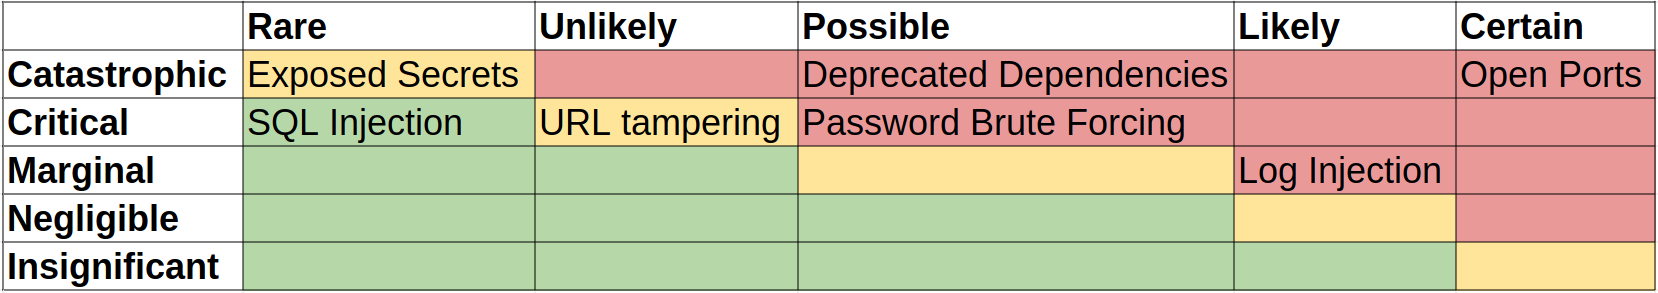
\includegraphics[width=1\linewidth]{images/risk-matrix.png}
    \caption{Risk matrix based on security assessment}
    \label{fig:enter-label}
\end{figure}
\subsubsection{Action Plan}
We discussed the results of the security assessment and decided on focusing on the risk scenarios placed in the red area of the risk matrix.

For the open ports, we went through our firewall settings and scanned our main server's IP address to see the current open ports. We tried to close the port we had open for Prometheus, but got conflicting results, when we checked the firewall istelf compared to the scan of the IP address.

For the log injection, we went through our code and ensured that all user data was sanitized before added to the log, such that it could not be tampered with.

For the depricated dependencies, we added the tool \textit{dependabot} to our CI/CD pipeline, which makes sure that the dependencies used in our Minitwit system are up to date and thereby less vulnerable to older known exploits.

For the password brute forcing, we decided to leave it as it, due to the group not having enough information on how the creation of users and login works in the simulator and thereby not knowing if the simulator could handle password restraints or 2-factor authentication, which could have been our solution to improve this issue.
